\subsubsection{Rationale/Context}
On special occasions or on short notice someone might need an urgent way of getting to one of  the islands. The taxi boat is a way of solving this problem.
\subsubsection{User story}
As a \textit{traveller}, I want to \textit{reserve} a boat taxi, from a given origin to a given destination, on a given time and date.
\subsubsection{Use Case}
\creator{\studentA}

\textbf{Use Case Name:} Reserve a taxi boat

\textbf{Scope:} Taxi reserving system

\textbf{Level:} User Goal

\textbf{Primary Actor:} Traveller

\textbf{Stakeholders and Interests:} 
\begin{itemize}
\item \textit{Traveller:} Wants to reserve a taxi boat for quick travel to one of the islands.
\item \textit{Seller:} Wants a platform that makes the reservation process easy, thus attracting clients.
\end{itemize}

\textbf{Preconditions:}
\begin{itemize}
\item The taxi boat is available on the selected time/hour/location combination.
\end{itemize}

\textbf{Success Guarantee (Postconditions):}
\begin{itemize}
    \item State change: The information about the taxi boat availability has been updated.
    \item Output: Information on the screen about the reservation and an unique code.
\end{itemize}

\textbf{Main Success Scenario (Basic Flow):}
\begin{enumerate}
\item The User indicates to the System, the wish to reserve the taxi boat.
\item The System sends the User a taxi boat reservation form with available departure times.
\item The User fills in the form: the date, the time, origin and destination.
\item The User sends the System the filled-in taxi boat reservation form.
\item The System checks whether the form is completed correctly (i.e., complete and error-free).
\item The System informs the User about its findings ("Ok" or indicating the gaps and errors found).
\item If the form is not completed correctly, steps 3 - 6 will be repeated.
\item The System generates a new, unique taxi boat reservation code.
\item The System stores all the information about the reservation.
\item The System generates shows the code to the screen with all the information related to the reservation.
\end{enumerate}

\textbf{Technology And Data Variations List:} 
\begin{itemize}
    \item Departure date: Date of the form DD/MM/YYYY
    \item Departure time: Time of the form HH:MM
    \item Destination name, Origin name: String chosen from a list
    \end{itemize}

\textbf{Frequency of Occurrence:} Few times a day, every day.

\subsubsection{SSD}
\creator{\studentA}
Considering the previous sub-sections we can create the following SSD model:\\\\
User $\rightarrow$ System: Reserve taxi boat;\hfill /* 1\\
System $\rightarrow$ User: Taxi boat reservation form;\hfill /* 2\\
repeat User $\rightarrow$ User: Fill in the form with: \underline{date of departure}, \underline{time of departure},\\ \underline{origin}, \underline{destination};\hfill /* 3\\
\phantom{x}\hspace{7mm} User $\rightarrow$ System: Filled-in Taxi boat reservation form;\hfill /* 4\\
\phantom{x}\hspace{7mm} System $\rightarrow$ System: Check whether the form is completed correctly; \hfill /* 5\\
\phantom{x}\hspace{7mm} System $\rightarrow$ User: "Ok" or the found gaps and errors;\hfill /* 6\\
until the form is completed correctly;\hfill /* 7\\
System $\rightarrow$ User: GenerateCode(date, time, origin, destination);\hfill /* 8\\
System $\rightarrow$ System: Store the information about the reservation;\hfill /* 9\\
System $\rightarrow$ User: Show the reservation code;\hfill /* 10\\

\subsubsection{Grey box SD}
\creator{\studentC}
\begin{figure}[H]
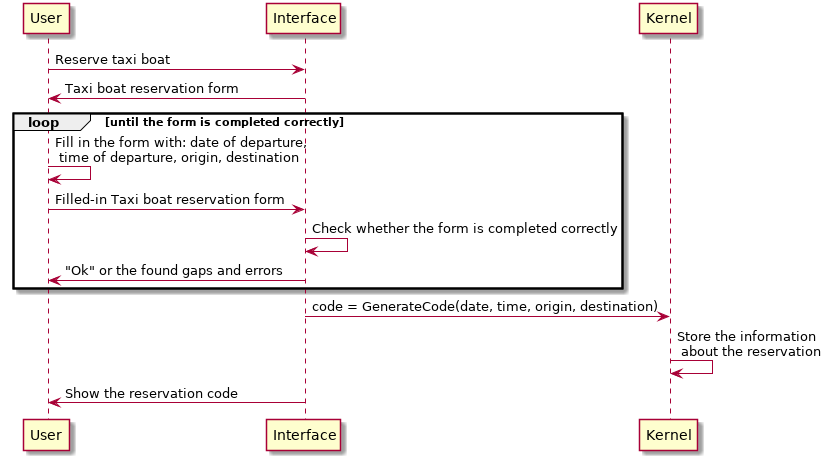
\includegraphics[scale=0.6]{Iteration_3/Files/UC6_gb.png}
\end{figure}
\iffalse
\begin{lrbox}{\mysavebox}%
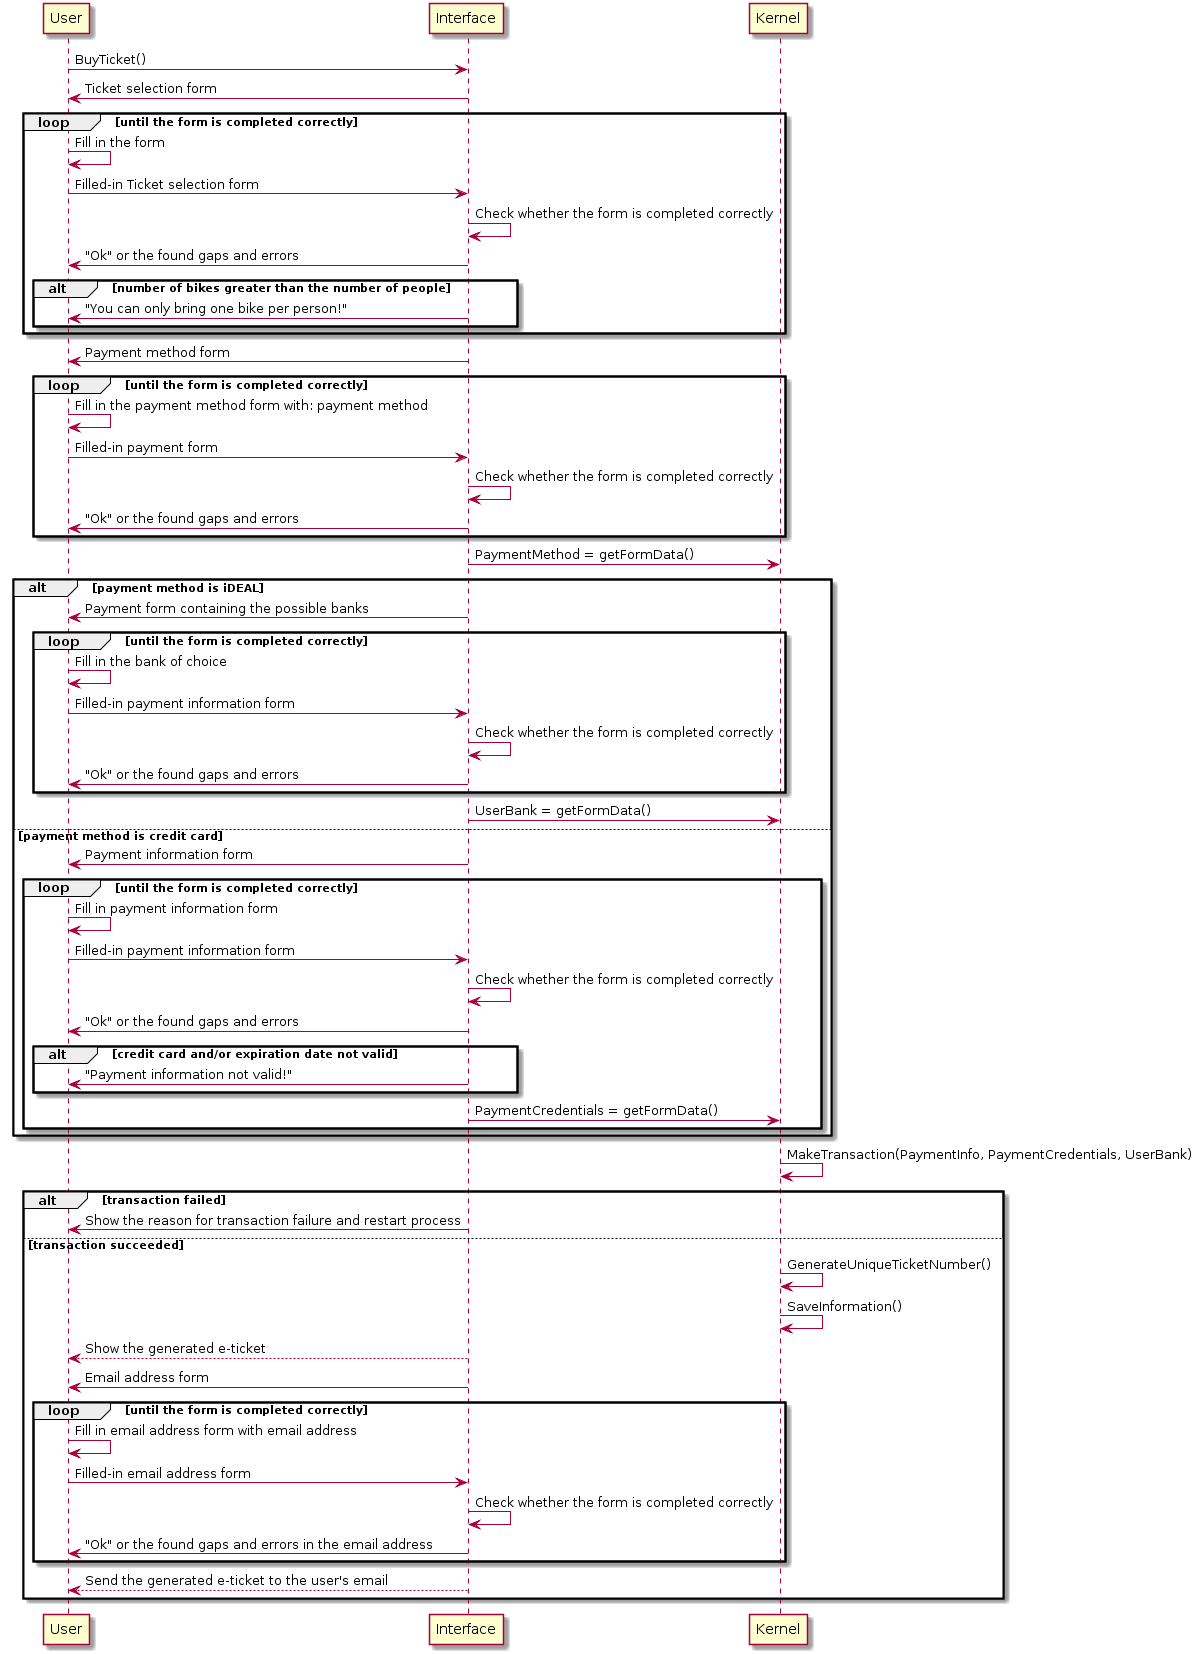
\includegraphics[scale=0.5]{Iteration_3/Files/UC1_gb.png}
\end{lrbox}
\fi

\ifdim\ht\mysavebox>\textheight
    \setlength{\myrest}{\ht\mysavebox}%
    \loop\ifdim\myrest>\textheight
        \newpage\par\noindent
        \clipbox{0 {\myrest-\textheight} 0 {\ht\mysavebox-\myrest}}{\usebox{\mysavebox}}%
        \addtolength{\myrest}{-\textheight}%
    \repeat
    \newpage\par\noindent
    \clipbox{0 0 0 {\ht\mysavebox-\myrest}}{\usebox{\mysavebox}}%
\else
    \usebox{\mysavebox}%
\fi

\subsubsection{White box SD}
\creator{\studentC}
\begin{figure}[H]
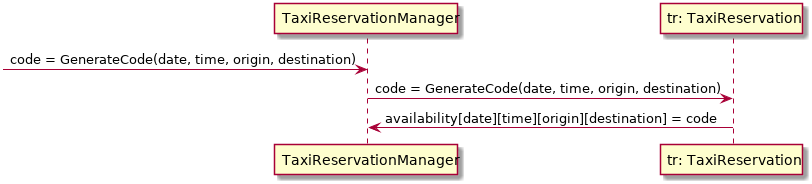
\includegraphics[scale=0.5]{Iteration_3/Files/UC6_wb.png}
\end{figure}
By not going into too many technical details, the kernel generates a code based on the data given (date, time, origin, destination) which is being used as a seed. Then, in the array containing the availability at the given params, the code is attached, so that we know that the taxi boat is reserved for that specific period.

\subsubsection{Design Considerations}
Because we didn't have a lot of details about this, and because work on it was started after the availability of Rob ceased to be present, we made some assumptions. These are:
\begin{itemize}
    \item The taxi boat can go from any location to any other location within the cities from the first part of the request from KOENDES (Harlingen, Terschelling, Vlieland).
    \item The payment will be made after the journey has ended.
    \item Considering a taxi is more personal, there is no need for mentioning the amount of people, since in most of the cases it shall be used by 2 people more or less.
\end{itemize}